\documentclass[compress]{beamer}
\usepackage[
    title={CVRP: MIP and Heuristic comparison},
    subtitle={Confronto tra modelli MIP e euristiche per il CVRP},
    event={Progetto fine corso AMOD},
    author={L. Falasca},
    longauthor={Luca Falasca},
    email={luca.falasca@students.uniroma2.eu},
    institute={Tor Vergata},
    longinstitute={Università degli Studi di Roma Tor Vergata},
]{unislides}
\usepackage{graphicx} % Required for inserting images
\usepackage{minted}
\usepackage{algorithm}
\usepackage{hyperref}
\usepackage{adjustbox}
\usepackage{svg}
%\svgsetup{inkscapelatex=false}

\begin{document}

\begin{frame}[plain]
	\titlepage
\end{frame}
\section{Introduzione}

\subsection{Obiettivi}
\begin{frame}{\subsecname}
    L'obiettivo di questo progetto è confrontare le prestazioni di un modello MIP e di alcune euristiche per la risoluzione del problema del Vehicle Routing Problem con capacità (CVRP).

    \begin{itemize}
        \item Implementazione di un modello MIP per il CVRP
        \item Implementazione di alcune euristiche per il CVRP
        \item Confronto delle prestazioni in termini di qualità della soluzione e tempo di esecuzione
    \end{itemize}
\end{frame}

\subsection{Dati e risorse tecniche}
\begin{frame}{\subsecname}
    \begin{itemize}
        \item Dati: set di benchmark Augerat 1995 e XML100 2021
        \item Software: Python (amplpy), AMPL, Gurobi
        \item Hardware: AMD Ryzen 5 7530U (6 core / 12 threads), 16 GB RAM
    \end{itemize}
\end{frame}

\section{Metodologia e Algoritmi}

\begin{frame}{Metodologia}
    \begin{itemize}
        \item Limite di tempo di 5 minuti (300 secondi) per ogni esecuzione
        \item Lower bound per il modello MIP
        \item Valutazione della distanza dalla soluzione ottima (Optimality Gap)
    \end{itemize}
\end{frame}

\subsection{Modello MIP}
\begin{frame}{\subsecname}
    \begin{itemize}
        \item Modello MIP b-matching relax (Miller 1995)
        \item Iterazione del modello MIP con aggiunta dinamica di vincoli fino alla soluzione ottima o al limite di tempo.
        \begin{itemize}
            \item Vincoli di sottociclo (subtour elimination constraints) 
            \item Vincoli di capacità (capacity constraints)
        \end{itemize}
        \item Uso di euristiche con grafi per trovare i vincoli dalla soluzione intermedia.
    \end{itemize}
\end{frame}

\subsection{Euristiche}

\subsubsection{Clarke and Wright}
    
\begin{frame}{\subsubsecname}
    \begin{itemize}
        \item Euristica di risparmio (savings)
        \begin{itemize}
            \item \( s(i,j) = c(0,i) + c(0,j) - c(i,j) \)
            \item Quanto mi conviene unire i nodi \(i\) e \(j\) in un unico percorso?
        \end{itemize}
        \item Calcolo del risparmio per ogni coppia di nodi
        \item Ordinamento decrescente dei risparmi
        \item Unione dei percorsi basata sui risparmi
    \end{itemize}

\end{frame}

\subsubsection{Sweep}
\begin{frame}{\subsubsecname}
    \begin{itemize}
        \item Ordinamento dei nodi in base all'angolo polare rispetto al deposito
        \item Creazione di percorsi sequenziali fino al raggiungimento della capacità del veicolo
    \end{itemize}
    \hfill
    \begin{minipage}{0.49\textwidth}
		\centering
		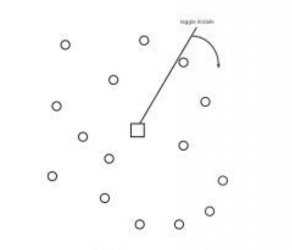
\includegraphics[width=0.8\linewidth]{images/sweep1.png}
	\end{minipage}
	\hfill
	\begin{minipage}{0.49\textwidth}
		\centering
		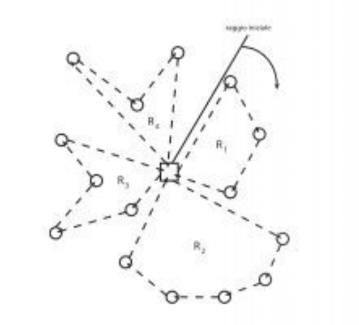
\includegraphics[width=0.8\linewidth]{images/sweep2.png}
	\end{minipage}
\end{frame}

\subsubsection{My Heuristic}
\begin{frame}{\subsubsecname}
    
    \begin{minipage}{0.49\textwidth}
        \begin{itemize}
        \item Variante del Nearest Neighbor
        \item Nodi vicini agli estremi
        \item Aggiunta iterativa di nodi al percorso
    \end{itemize}
    \end{minipage}
    \begin{minipage}{0.49\textwidth}
        \centering
        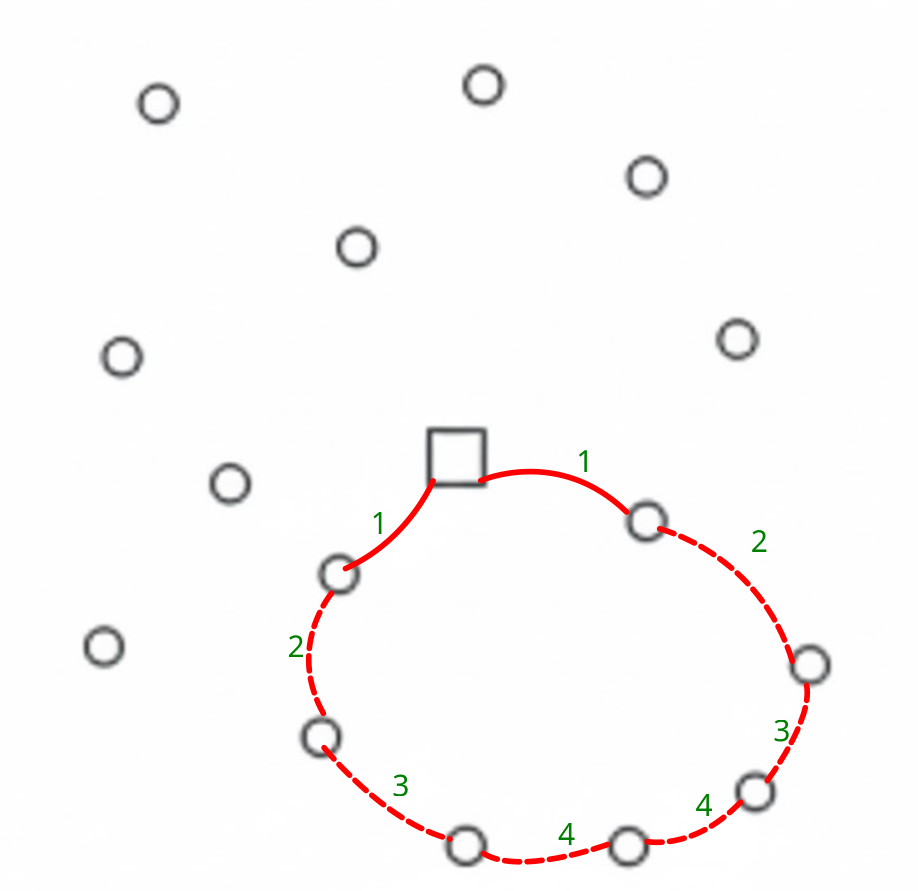
\includegraphics[width=0.8\linewidth]{images/my_heuristic.png}
    \end{minipage}
\end{frame}

\section{Risultati}

\subsection{Augerat 1995}

\begin{frame}{\subsecname}
    \begin{center}
        \begin{itemize}
            \item 28 istanze di test
            \item N variabile tra 31 e 80
            \item K variabile tra 5 e 10
        \end{itemize}
    \end{center}
\end{frame}

\begin{frame}{\subsecname}
    \begin{center}
		\begin{minipage}{1\textwidth}
            \centering
            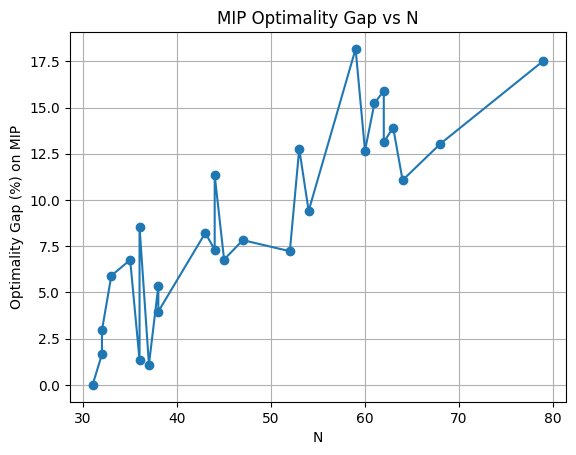
\includegraphics[width=0.75\linewidth]{images/MIP.png}
        \end{minipage}
    \end{center}
\end{frame}

\begin{frame}{\subsecname}
    \begin{center}
		\begin{minipage}{1\textwidth}
            \centering
            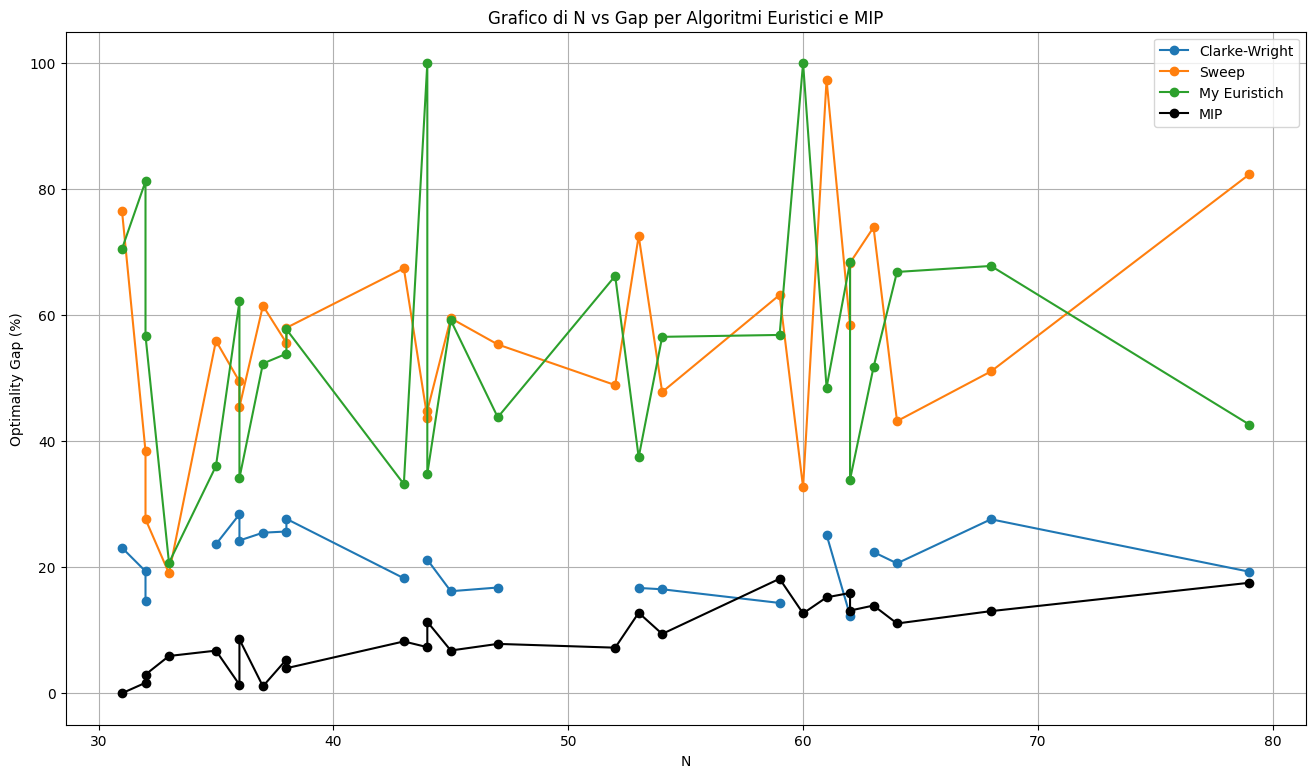
\includegraphics[width=1\linewidth]{images/N_gap.png}
        \end{minipage}
    \end{center}
\end{frame}

\begin{frame}{\subsecname}
    \begin{center}
		\begin{minipage}{1\textwidth}
            \centering
            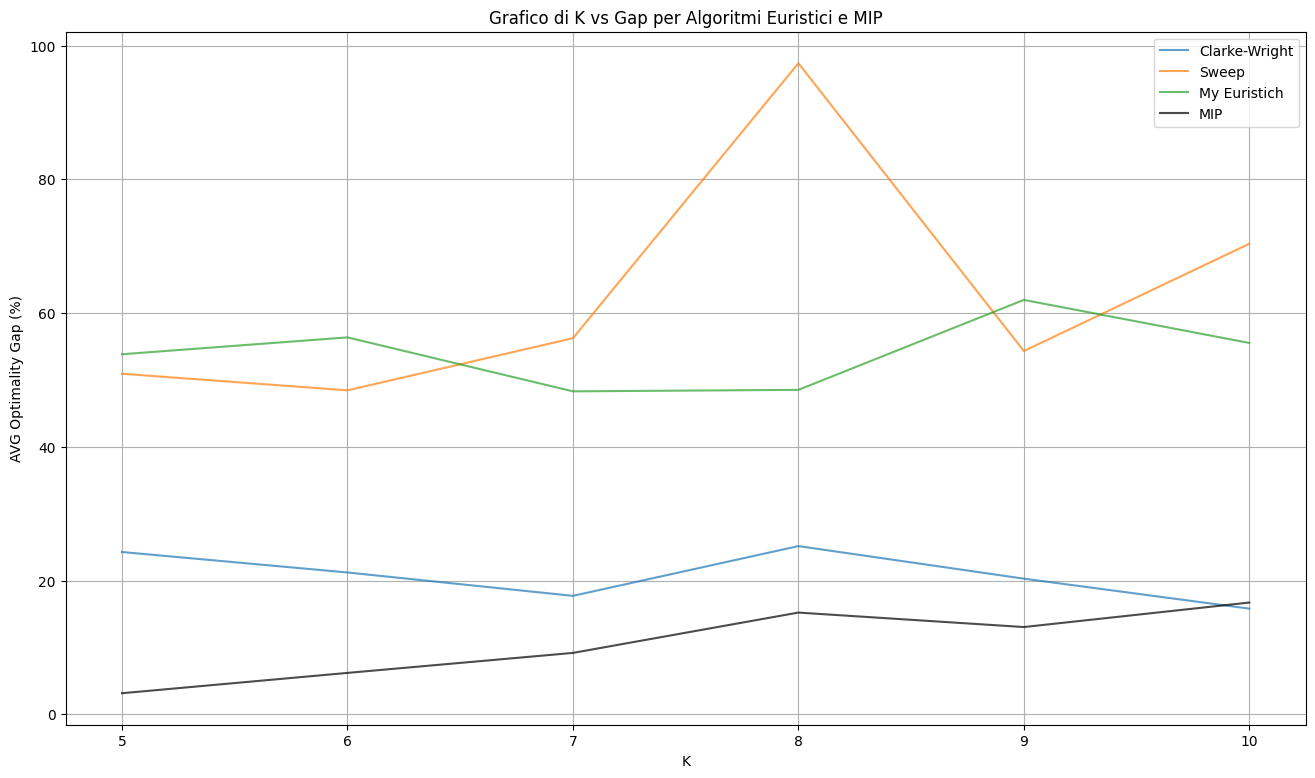
\includegraphics[width=1\linewidth]{images/K_gap.png}
        \end{minipage}
    \end{center}
\end{frame}

\begin{frame}{\subsecname}
    \begin{center}
		\begin{minipage}{1\textwidth}
            \centering
            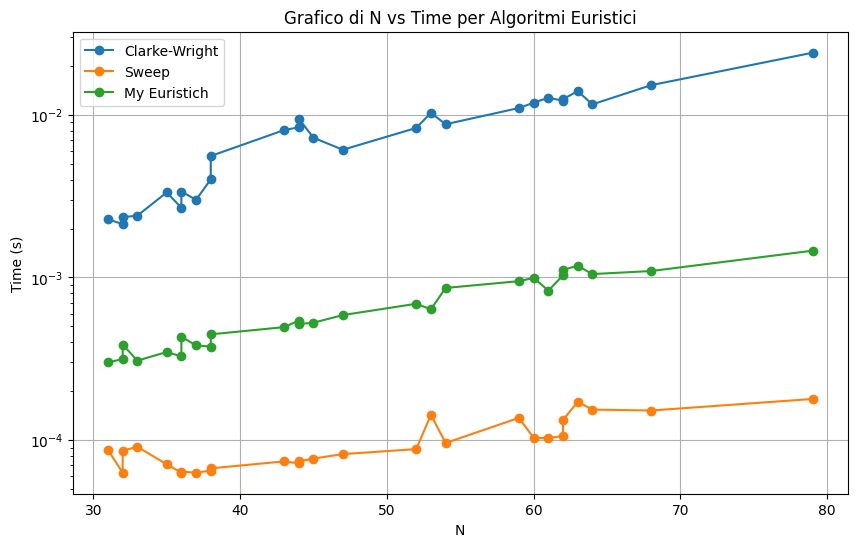
\includegraphics[width=1\linewidth]{images/N_time.png}
        \end{minipage}
    \end{center}
\end{frame}

% \begin{frame}{\subsecname}
%     \begin{center}
% 		\begin{minipage}{1\textwidth}
%             \centering
%             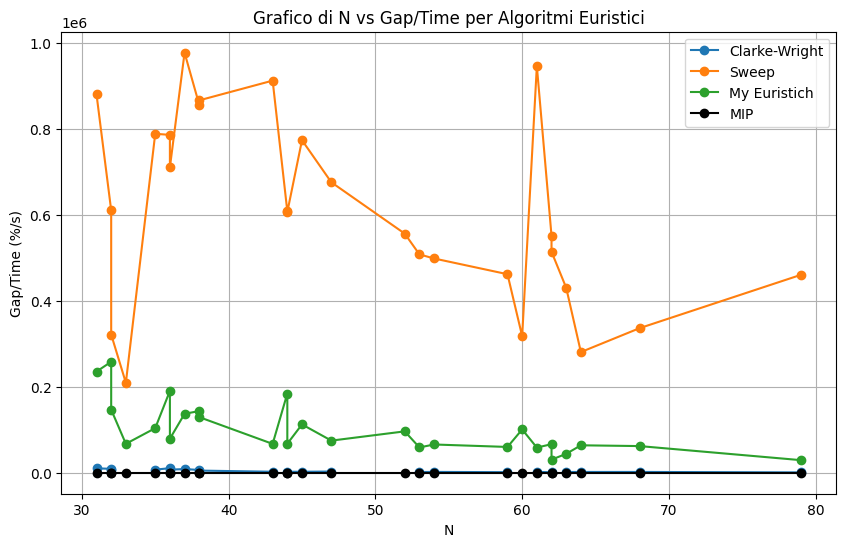
\includegraphics[width=1\linewidth]{images/N_gap_over_time.png}
%         \end{minipage}
%     \end{center}
% \end{frame}

\begin{frame}{\subsecname}
    \begin{center}
		\begin{minipage}{1\textwidth}
            \centering
            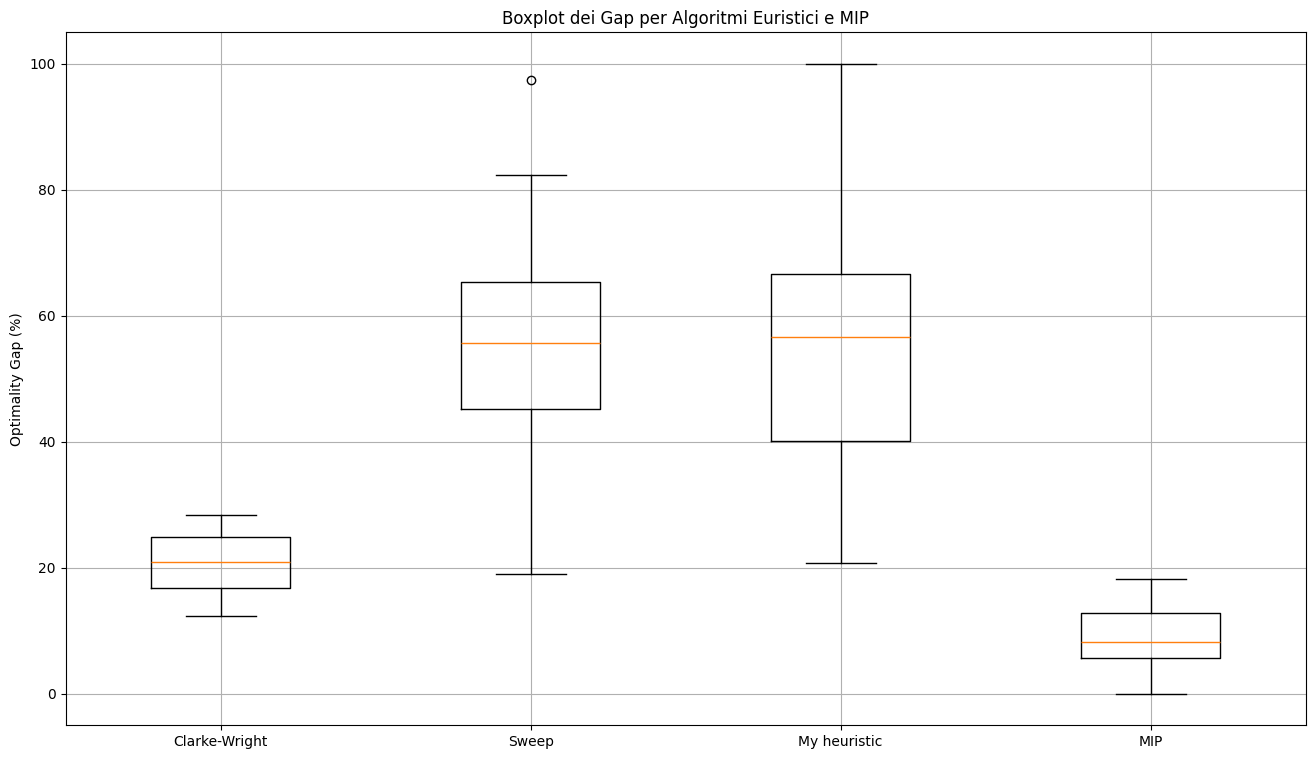
\includegraphics[width=1\linewidth]{images/boxplot_gap.png}
        \end{minipage}
    \end{center}
\end{frame}


\subsection{XML100 2021}

\begin{frame}{\subsecname}
    \begin{center}
        \begin{itemize}
            \item 10000 istanze di test
            \item N = 100
            \item K non fisso, dipende dall'istanza
            \item Varie tipologie di istanze
        \end{itemize}

        \begin{minipage}{0.9\textwidth}
            \centering
            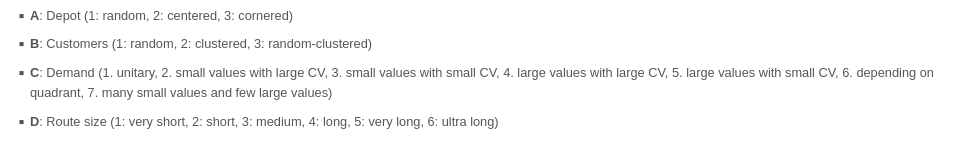
\includegraphics[width=1\linewidth]{images/xml100_types.png}
        \end{minipage}
    \end{center}
\end{frame}

\begin{frame}{\subsecname}
    \begin{center}
		\begin{minipage}{1\textwidth}
            \centering
            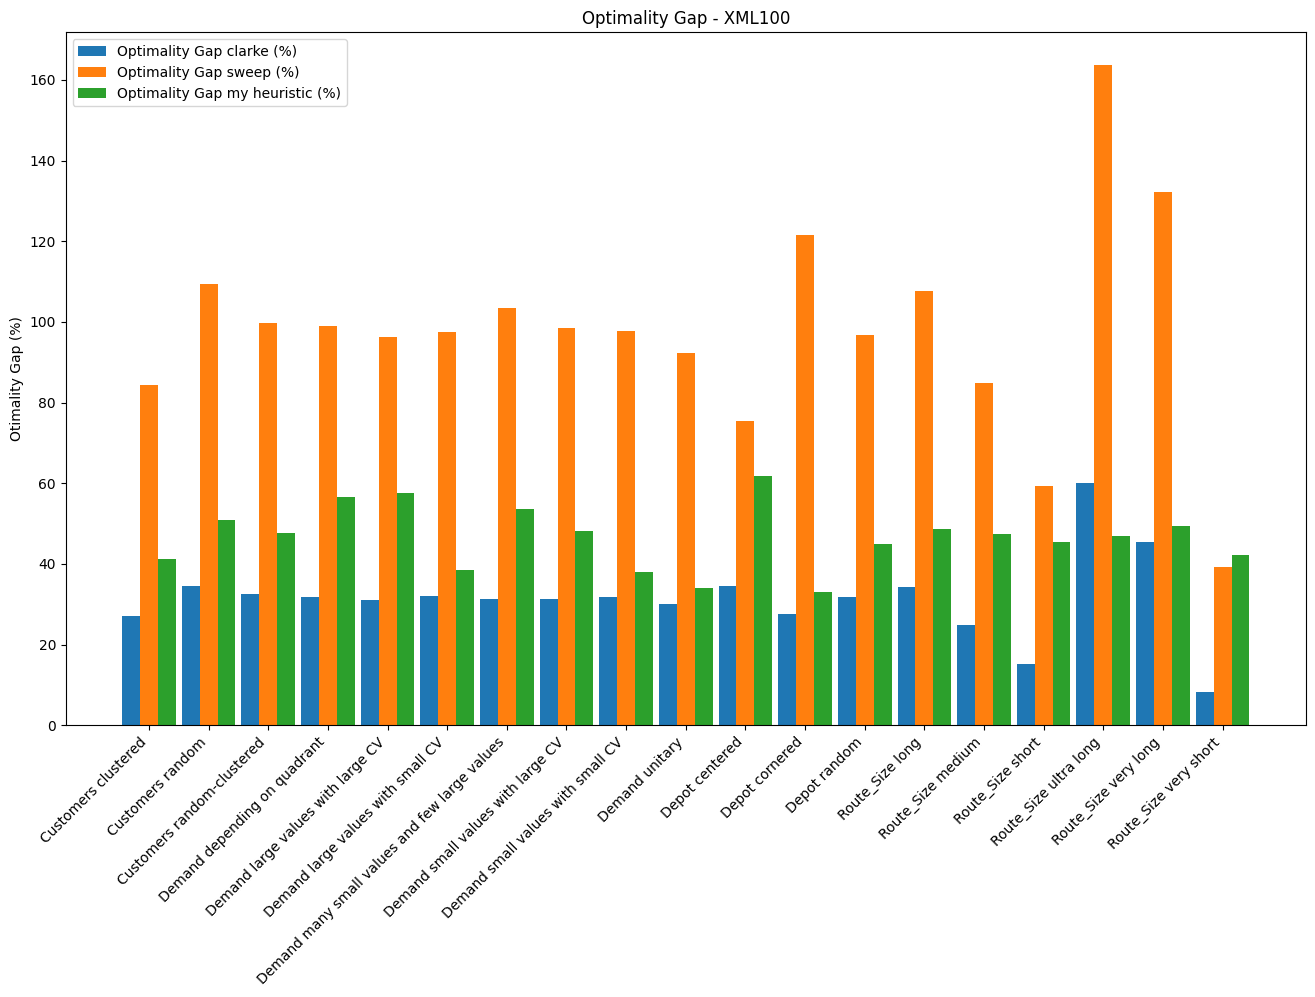
\includegraphics[width=0.8\linewidth]{images/xml100_gap.png}
        \end{minipage}
    \end{center}
\end{frame}

\begin{frame}{\subsecname}
    \begin{center}
		\begin{minipage}{1\textwidth}
            \centering
            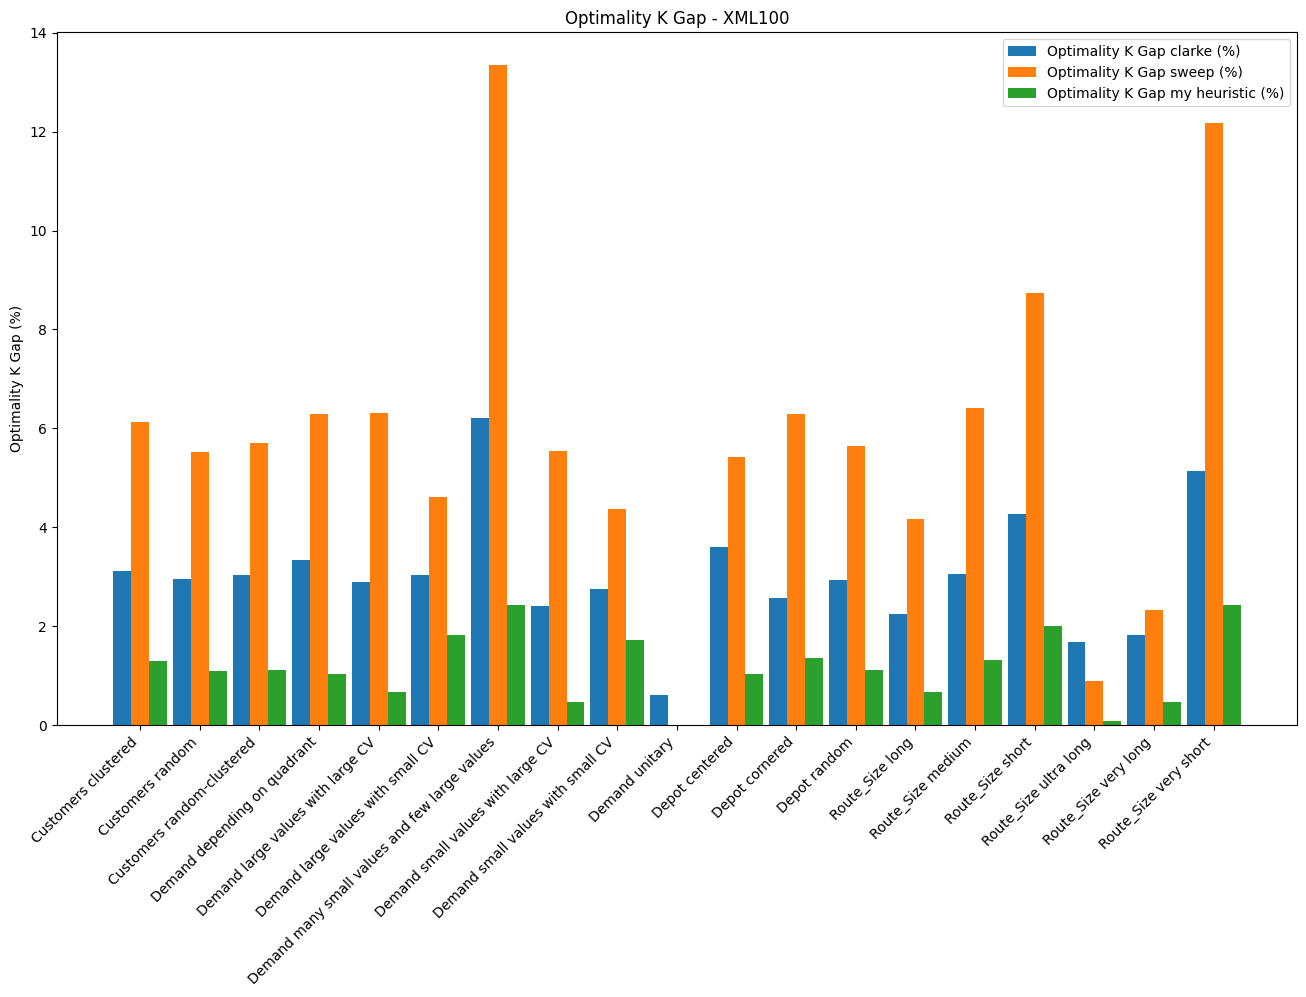
\includegraphics[width=0.8\linewidth]{images/xml100_kgap.png}
        \end{minipage}
    \end{center}
\end{frame}

\begin{frame}{\subsecname}
    \begin{center}
		\begin{minipage}{1\textwidth}
            \centering
            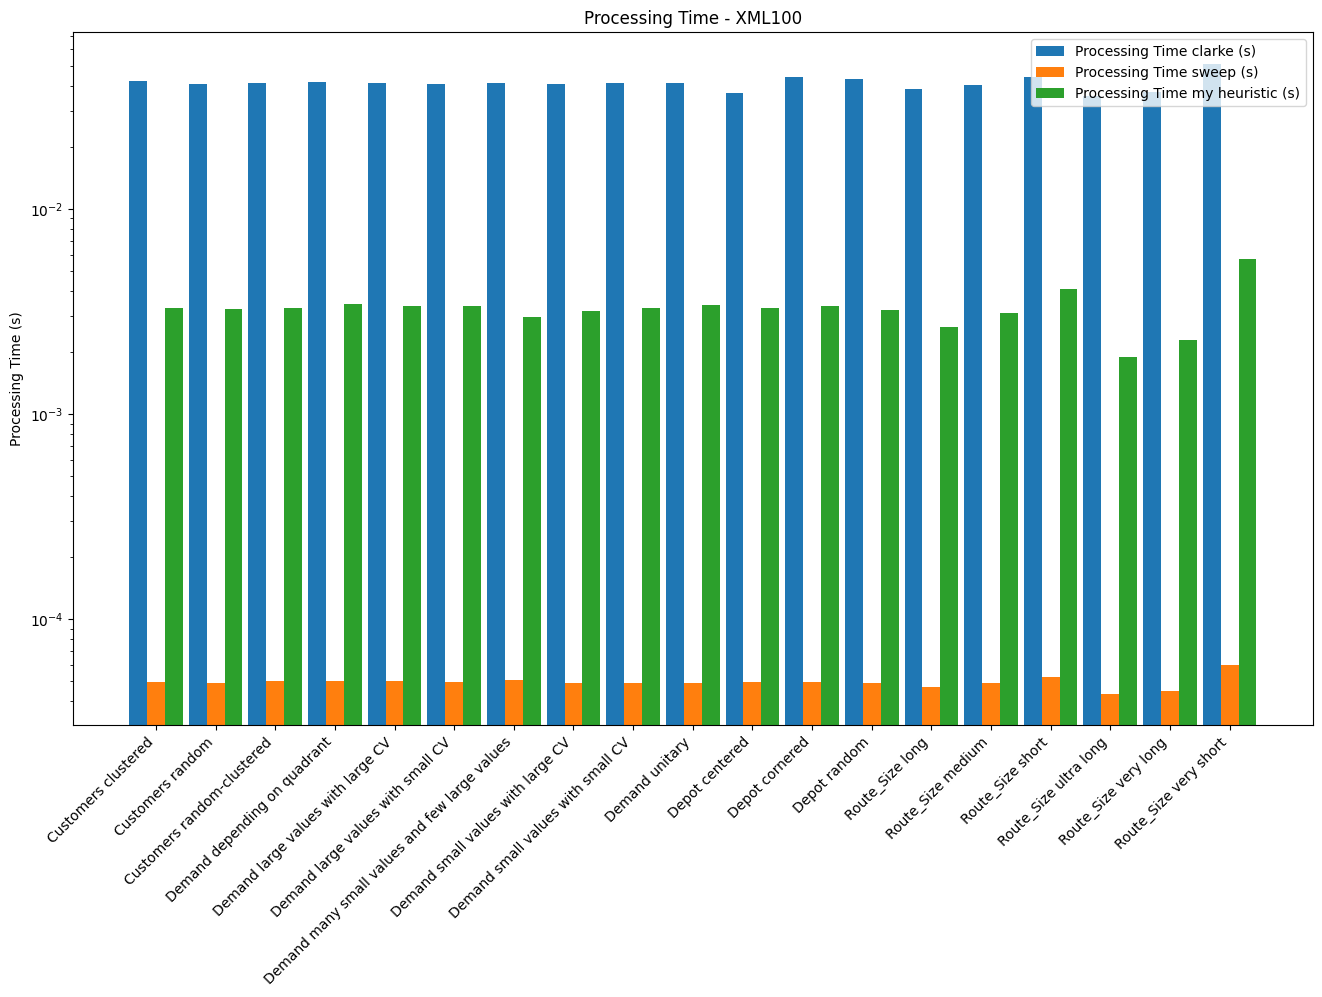
\includegraphics[width=0.8\linewidth]{images/xml100_time.png}
        \end{minipage}
    \end{center}
\end{frame}

\begin{frame}{\subsecname}
    \begin{center}
		\begin{minipage}{1\textwidth}
            \centering
            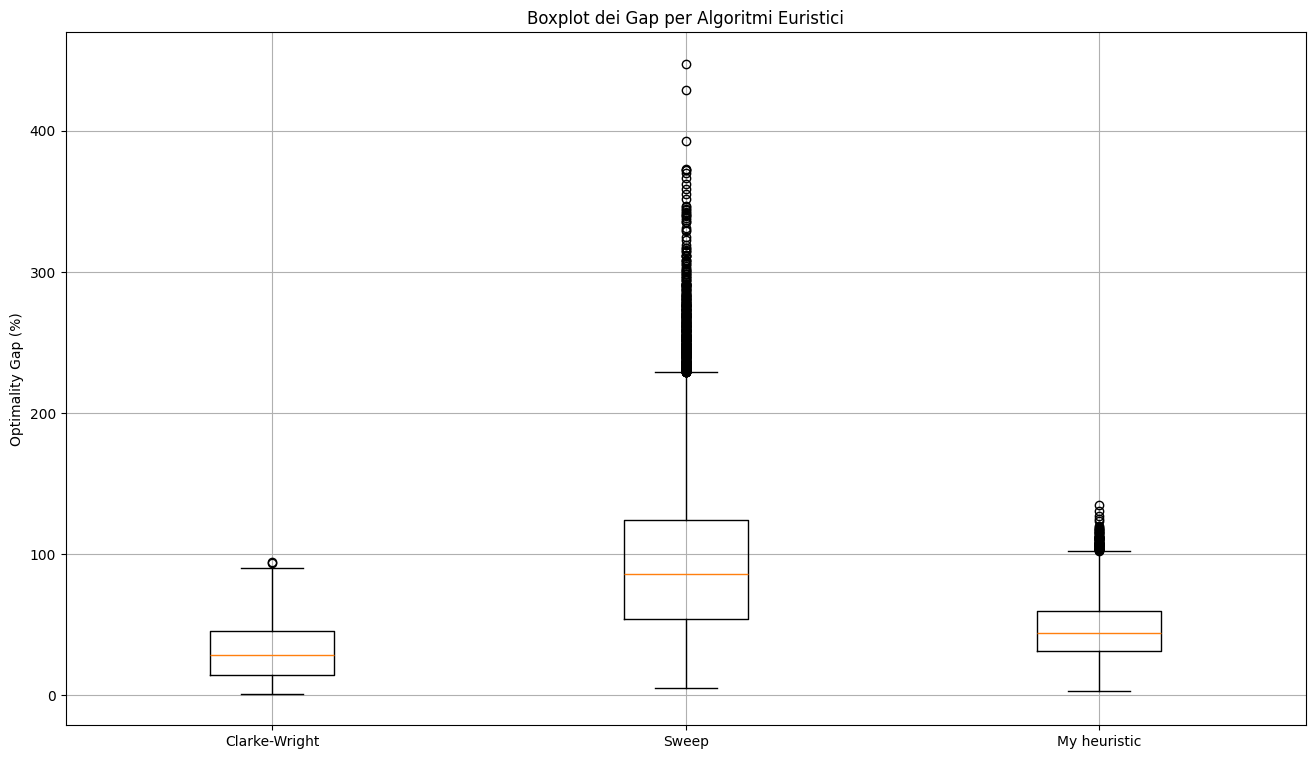
\includegraphics[width=1\linewidth]{images/xml100_boxplot.png}
        \end{minipage}
    \end{center}
\end{frame}

\begin{frame}
	\frametitle{Grazie per l'attenzione!}
	\begin{Huge}
		Domande?
	\end{Huge} 
	\\ \\
	Il codice è disponibile al seguente repository: \url{https://github.com/LucaFalasca/CVRP-PLI-Euristich-Compare}
	\\ \\
	
\end{frame}

\end{document}
